% This tutorial is created by Denis Stepanov, June 2020

\chapter{SHORT Template Tutorial}
\label{ch:tutorial}
Read this section if you are unfamiliar with \LaTeX, Overleaf, or formatting templates in general. If you think you are smart and ready-to-go, comment out the include statement of this chapter in body file and move on. You can delete it too if you want :)

\section{Intr0}
Your project will include chapters, sections and subsections. To start writing a chapter, create a separate file in the body folder and use this commands:

\begin{verbatim}
\chapter{New Chapter}
\label{chapter:myNewChapter}
\end{verbatim}

Always include labels as you would need them later to references different parts of your paper. For example this chapter's label is ``ch:tutorial''. To reference this chapter you need to do this:

\begin{verbatim}
Chapter \ref{ch:tutorial} is cool.
\end{verbatim}

The out output will be generated with the number that is referenced by your chapter. Everything is auto generated, so you do no have to worry about naming everything by hand. \LaTeX{} will do everything for you:

Chapter \ref{ch:tutorial} is cool. 

Similarly, you can create sections, subsections, and sub-subsections. Use this as an example:

\begin{verbatim}
\section{Cool Introduction Section}
\label{sec:cool_intro}

\subsection{Cool Introduction Subsection}
\label{sec:cool_intro_subsec}

\subsubsection{Cool Introduction Sub-subsection}
\label{sec:cool_intro_subsubsec}
\end{verbatim}

Compiled documented with those lines will look like this:

\section{Cool Introduction Section}
\label{sec:cool_intro}

\subsection{Cool Introduction Subsection}
\label{sec:cool_intro_subsec}

\subsubsection{Cool Introduction Sub-subsection}
\label{sec:cool_intro_subsubsec}

Also, check your Table of Contents (TOC) at the top. You can see that everything is automatically added to it and you can click on it (hyperlink) to jump straight to that part of the text in the paper.

\section{Fil3s}
This templates includes multiple files that make this whole project work. Be sure to remember what you modify and note it as a comment (\% sign at the beginning of the line) because if you break something...it could be hard to find later.

So, this template includes:
\begin{itemize}
    \item Abbreviations - list of all your abbreviations, please use it!
    \item Appendices - include all your appendices there, such as source code samples, additional information about your project, further readings.
    \item Bibliography - your references go there. We will talk about formatting them later.
    \item Body - ALL your body files should go there. Trust me, it is for your own good to keep them separately from others.
    \item Images - I hope it is self-explanatory folder.
    \item Listings - Your source code files, if you would have any. We will talk about them later too.
    \item Preface - Everything that goes before the TOC.
    \item Preamble - your package files. Be sure to keep track of what you are adding/removing in that file!
    \item thesis.sty - Styling file for title page and preface. You can read more comments there.
    \item thesis.tex - Your ``main'' file of the project. Start there.
\end{itemize}

Most of these files are self-explanatory and easy to understand with some ``Googling''. If you have any problems, make sure that you always keep a copy of your project somewhere safe.

\section{F0rm4tting}
This section introduces you to some simple formatting techniques that you might be unfamiliar with if using \LaTeX{} for the first time.

\subsection{Lists}
Numbered list:
\begin{verbatim}
\begin{enumerate}
    \item item 0
    \item item 1
\end{enumerate}
\end{verbatim}
Bullets:
\begin{verbatim}
\begin{itemize}
    \item item 0
    \item item 1
\end{itemize}
\end{verbatim}

\subsection{Quotes: How to use it right}
``hello world'' vs. "hello world"

Google this. Thank me later.

\subsection{T3xt}
Format your text with these command by including the text that needs to be formatted in the curly brackets:

\begin{verbatim}
\textbf{Bold}
\textit{Italic}
\texttt{Typewriter}
\textsc{Small Caps}
\end{verbatim}

\subsection{F1gur3s}
All figures you create in this project will be automatically added to the list of figures. There are several formatting techniques you can do to your images. For example if your images are too large you can scale it:

\begin{verbatim}
\begin{figure}
    \centering
    
\includegraphics[scale=1.0]{images/nottingham-logo.png}
    \caption{UNNC Logo Original}
    \label{fig:logo1}
\end{figure}

\begin{figure}
    \centering
    
\includegraphics[scale=0.5]{images/nottingham-logo.png}
    \caption{UNNC Logo Formatted}
    \label{fig:logo2}
\end{figure}
\end{verbatim}

Commands above produce the following output:
\begin{figure}[H]
    \centering
    
\includegraphics[scale=1.0]{images/nottingham-logo.png}
    \caption{UNNC Logo Original}
    \label{fig:logo1}
\end{figure}

\begin{figure}[H]
    \centering
    
\includegraphics[scale=0.5]{images/nottingham-logo.png}
    \caption{UNNC Logo Formatted}
    \label{fig:logo2}
\end{figure}

You can also move the position of the picture on the page, but I prefer to use [H] option (put at that specific place), even if sometimes it is not optimal. I let you search other options by yourself.

Another example is placing two figures side by side. Make sure they are same size (width x length):

\begin{verbatim}
\begin{figure}[H]
\centering
\begin{minipage}{.5\textwidth}
  \centering
  
\includegraphics[width=.8\linewidth]{images/nottingham-logo.png}
  \captionof{Figure \#2}
  \label{fig:fig1}
\end{minipage}%
\begin{minipage}{.5\textwidth}
  \centering
  
\includegraphics[width=.8\linewidth]{images/nottingham-logo.png}
  \caption{Figure \#1}
  \label{fig:fig2}
\end{minipage}
\end{figure}
\end{verbatim}

The commands above produce output like this:

\begin{figure}[H]
\centering
\begin{minipage}{.5\textwidth}
  \centering
  
\includegraphics[width=.8\linewidth]{images/nottingham-logo.png}
  \caption{Figure \#1}
  \label{fig:fig1}
\end{minipage}%
\begin{minipage}{.5\textwidth}
  \centering
  
\includegraphics[width=.8\linewidth]{images/nottingham-logo.png}
  \caption{Figure \#2}
  \label{fig:fig2}
\end{minipage}
\end{figure}

Ideally, you should also reference it properly in your text:

\begin{verbatim}
Figures \ref{fig:fig1} & \ref{fig:fig2} show UNNC logo.
\end{verbatim}

which displays as: Figures \ref{fig:fig1} \& \ref{fig:fig2} show UNNC logo.

Pro-tip: in my project I had to include timeline of my dissertation, but it couldn't fit in the page, especially when there are two separate timelines in the project (original \& modified). The tip is to use landscape mode: make it on a separate page with the images of your timelines (probably created using some MS tools).

\begin{verbatim}
\clearpage
\begin{landscape}
\begin{figure}[H]
    \centering
    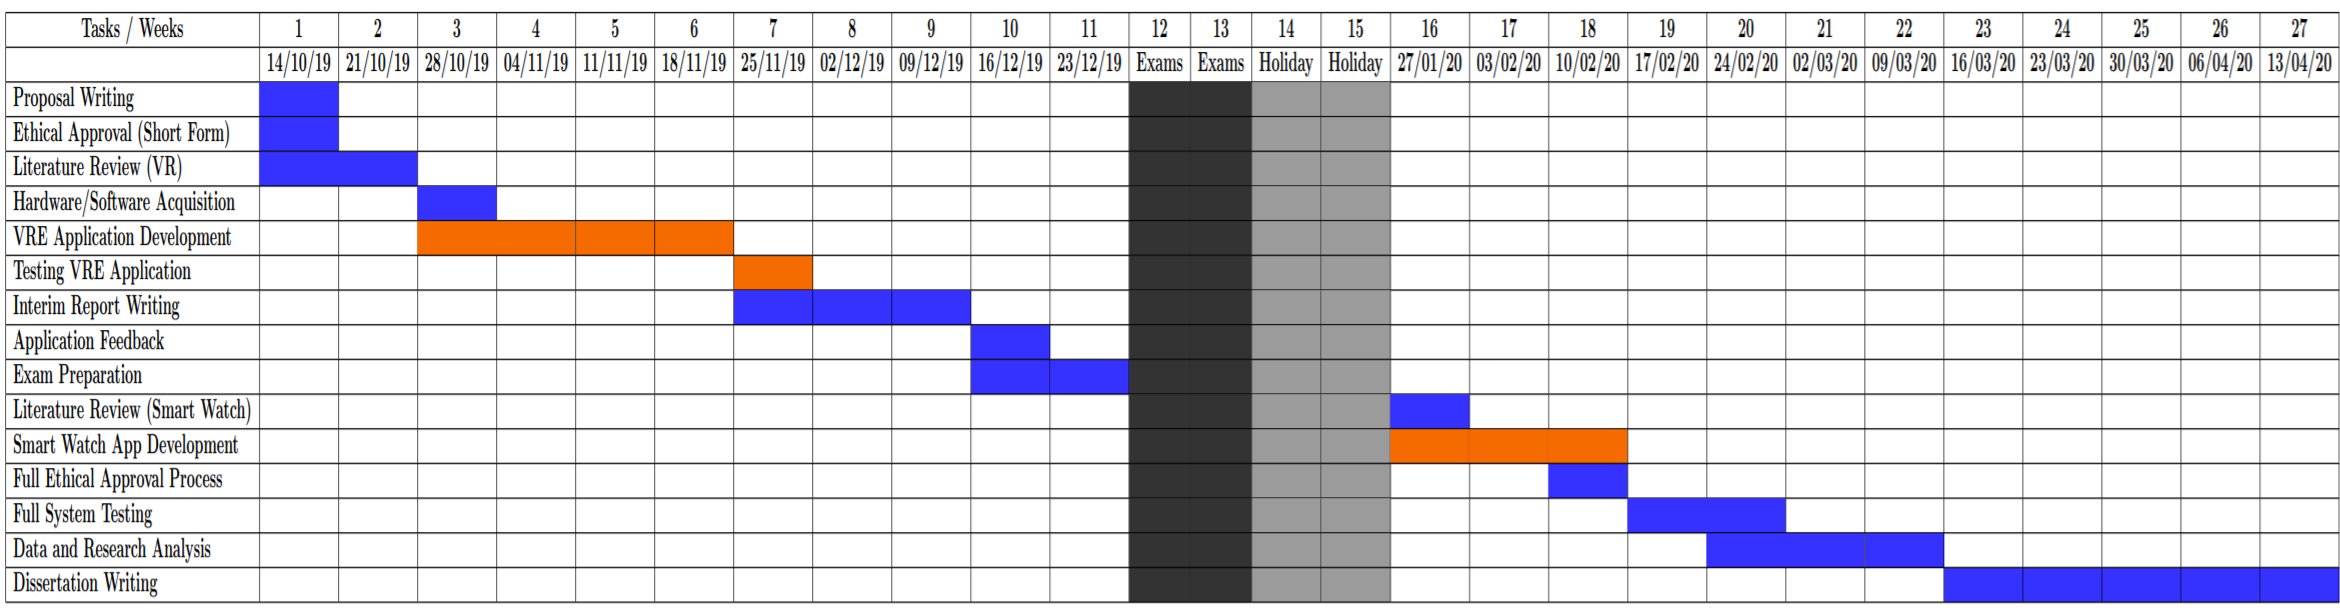
\includegraphics[scale=0.4]{images/chart.png}
    \caption{Original Timeline}
    \label{fig:chart}
\end{figure}

\begin{figure}[H]
    \centering
    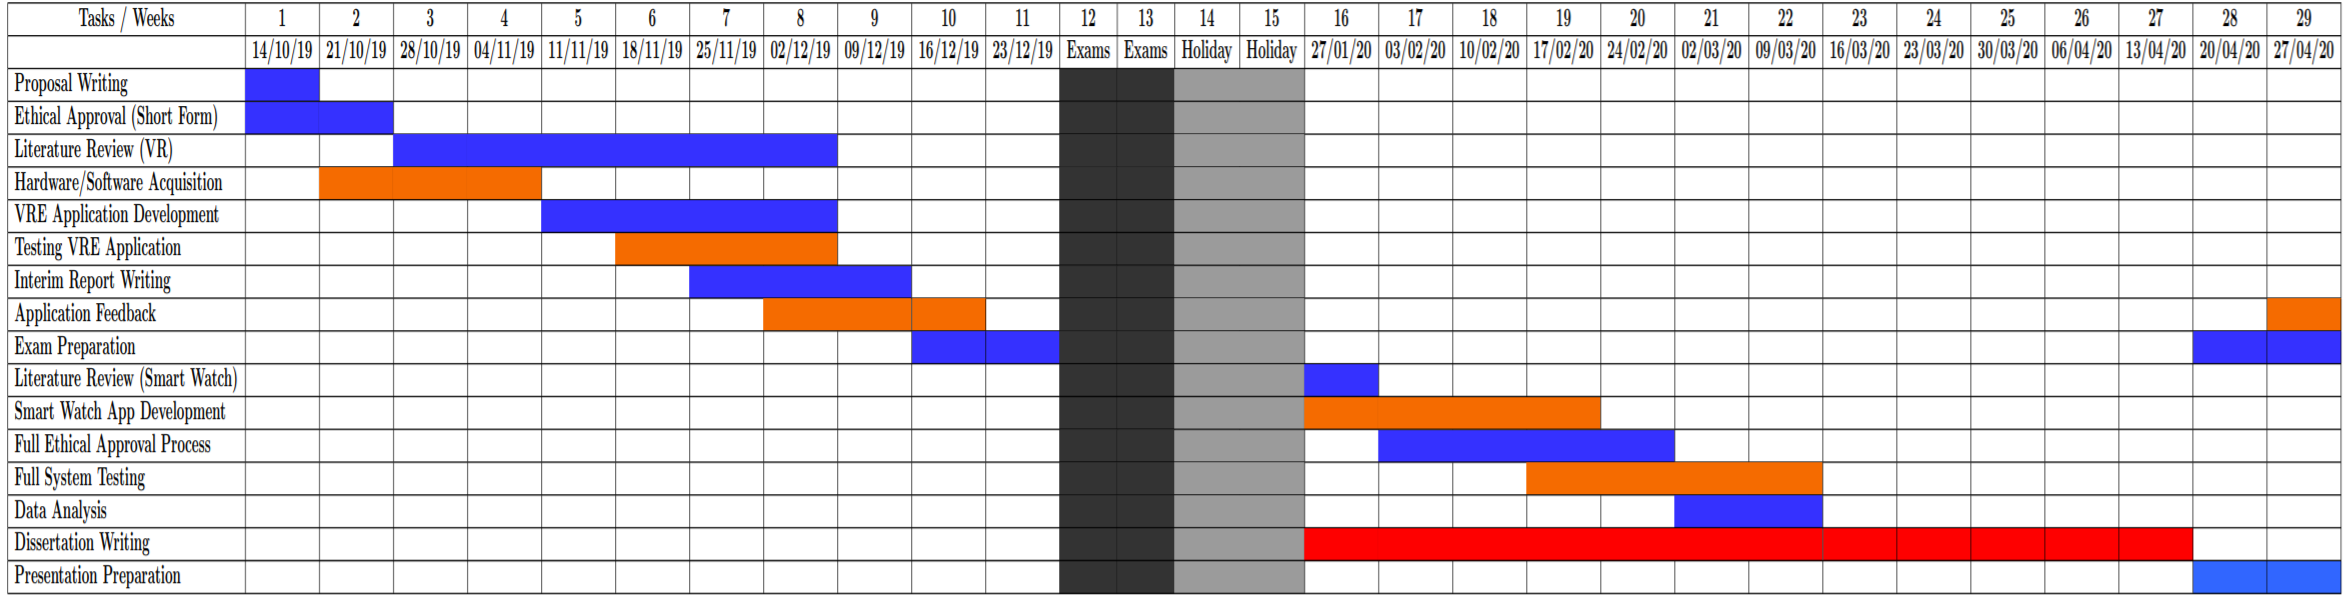
\includegraphics[scale=0.4]{images/new_chart.png}
    \caption{Updated Timeline}
    \label{fig:new_chart}
\end{figure}

\end{landscape}
\end{verbatim}

\begin{landscape}
\begin{figure}[H]
    \centering
    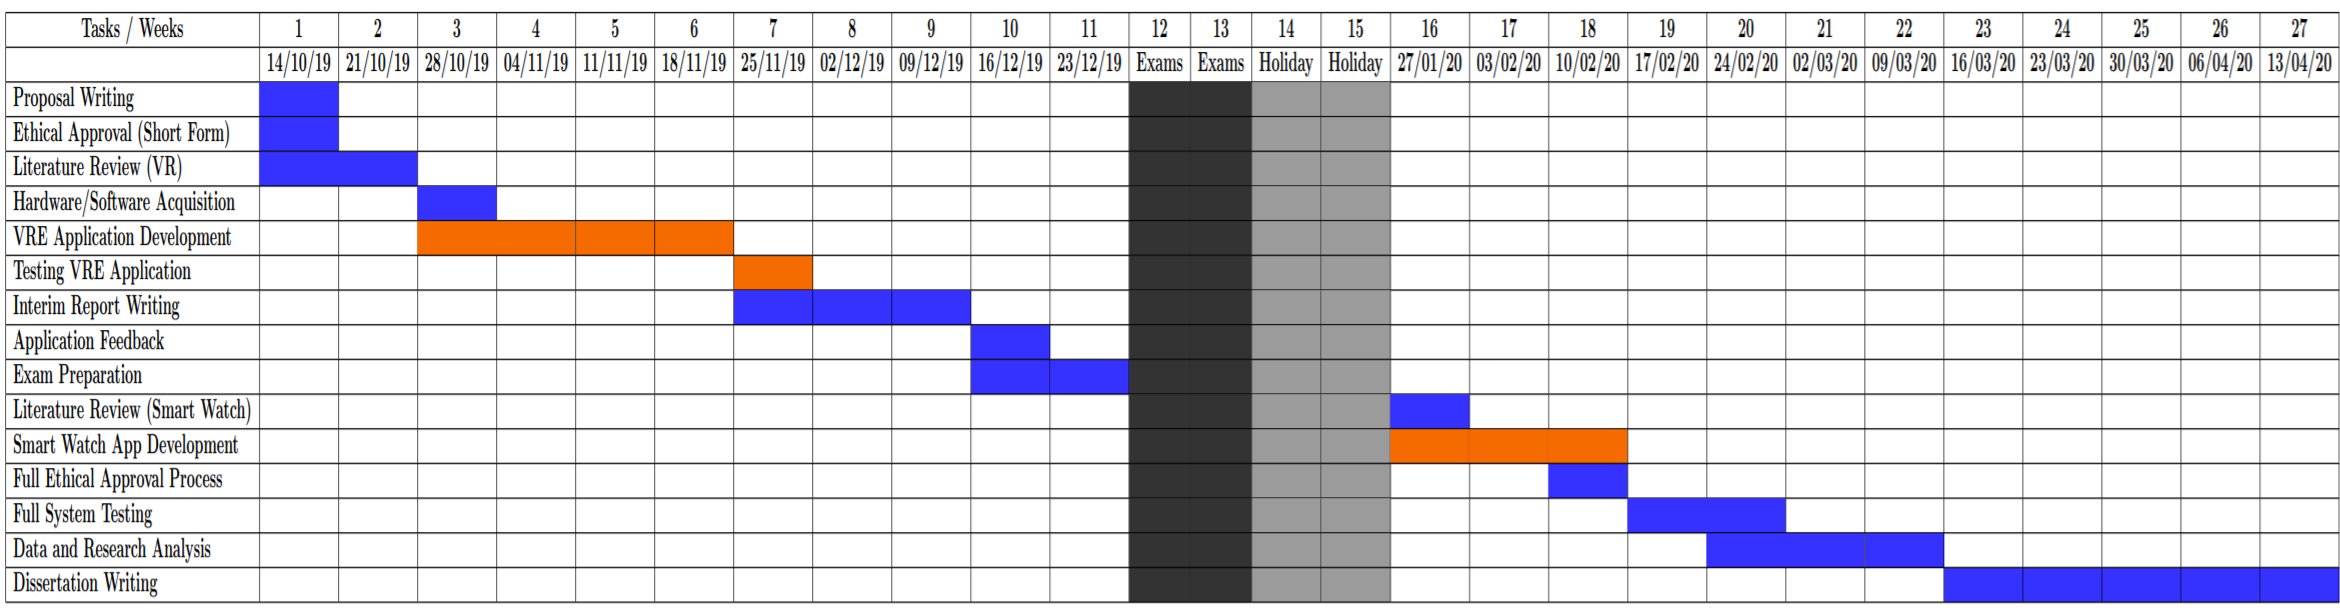
\includegraphics[scale=0.4]{images/chart.png}
    \caption{Original Timeline}
    \label{fig:chart}
\end{figure}

\begin{figure}[H]
    \centering
    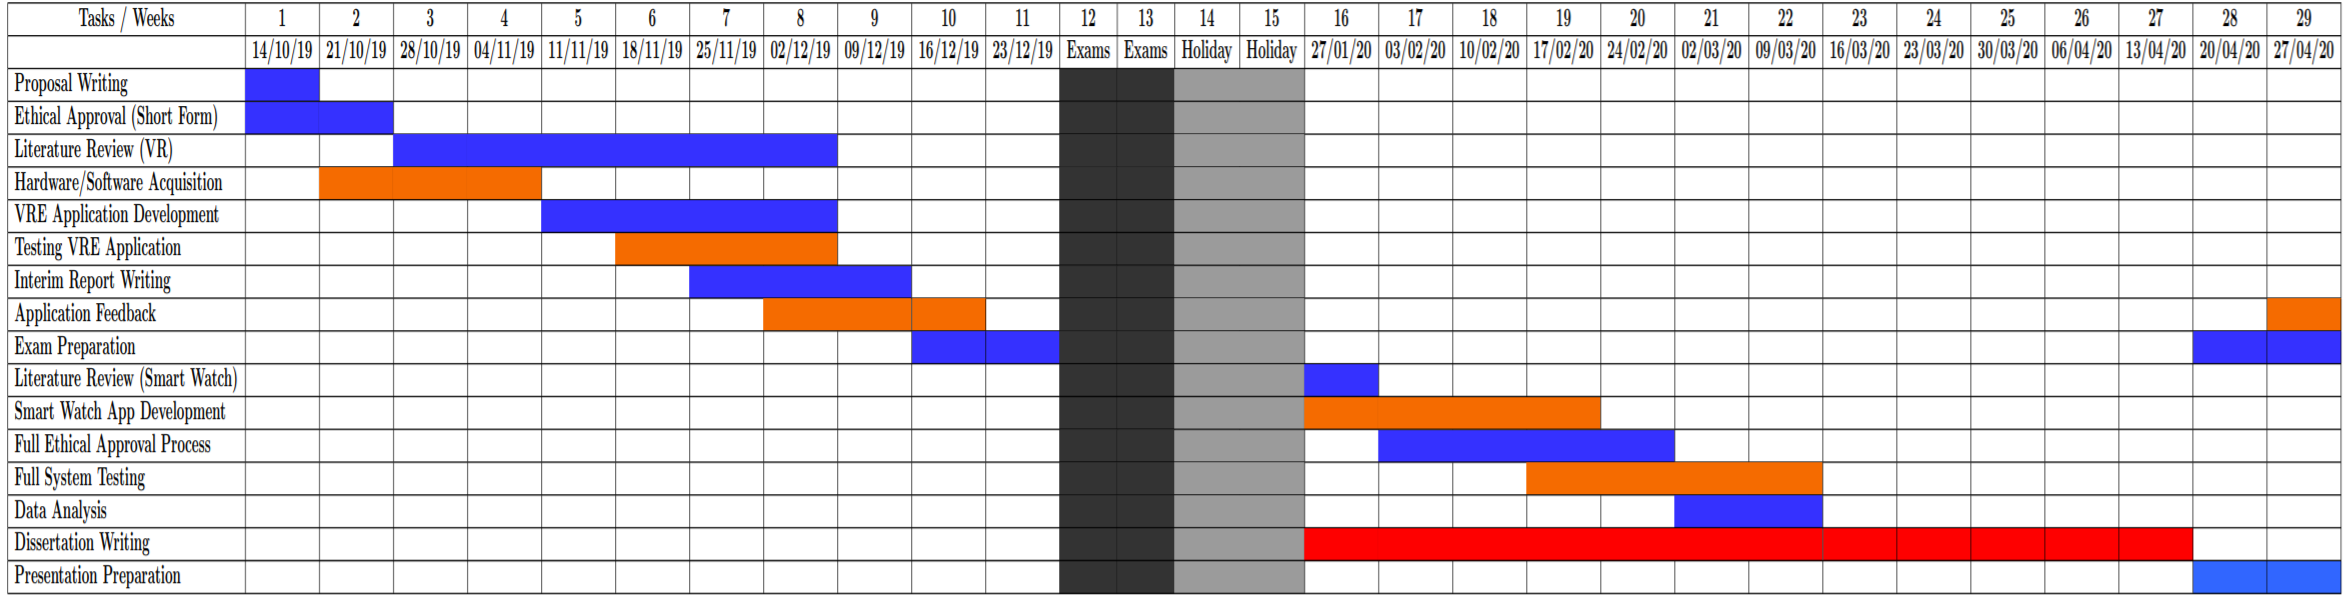
\includegraphics[scale=0.4]{images/new_chart.png}
    \caption{Updated Timeline}
    \label{fig:new_chart}
\end{figure}

\end{landscape}

\subsection{T4bles}
Tables are simple. Follow the format below to create your custom table. But, beware of the paper size: sometimes table might need scaling! The table will be also added to the list of tables after your TOC, same as figures.

\begin{verbatim}
\begin{table}[H]
\centering
\begin{tabular}{|c|c|c|}
\hline
ID & Fruit & Color     \\ \hline
1 & Apple & Red        \\ \hline
2 & Banana & Yellow    \\ \hline
3 & Watermelon & Green \\ \hline
4 & Orange & Orange    \\ \hline
\end{tabular}
\caption{Fruits}
\label{tab:tableFruits}
\end{table}
\end{verbatim}

\begin{table}[H]
\centering
\begin{tabular}{|c|c|c|}
\hline
ID & Fruit & Color     \\ \hline
1 & Apple & Red        \\ \hline
2 & Banana & Yellow    \\ \hline
3 & Watermelon & Green \\ \hline
4 & Orange & Orange    \\ \hline
\end{tabular}
\caption{Fruits}
\label{tab:tableFruits}
\end{table}

You can also check table generators online, there are plenty!

\subsection{L1st1ngs}
Sometimes you might want to include code samples in your report.

\begin{verbatim}
\lstinputlisting[language=Octave, caption=Code Sample]{hello_world.m}
\end{verbatim}

\lstinputlisting[language=Octave,caption=Code Sample]{listings/hello_world.m}

\section{Ref3rences}
Creating bibliography (properly) might be annyoing and hard, but, if you do it right from the beginning, then it should not be a problem. All your references should be stored in bibliography file and called from \textbf{thesis.tex} file in the end. Pay attention to what style you are using because it might affect the output - the displaying format of your citations.

So, let's take an example from my project's publications section:

\begin{verbatim}
One paper was accepted to appear in... \cite{compsac}.
\end{verbatim}

One paper was accepted to appear in... \cite{compsac}.

Check the references file. It will be all auto-generated. Pay attention to references names, author names, titles, dates, etc. Always check what format you use for citations as in \textbf{inbook}, \textbf{inproceedings}, \textbf{misc}, or other. More information you can find online. \href{https://www.overleaf.com/learn/latex/bibliography_management_with_bibtex}{(CLICK ME)}


\section{Summ4ry}
Here are some additional commands that you might use in your project:

\begin{verbatim}
\nth{4} - appends th to a number
\clearpage - clears the page, the text will continue on other page
\cleardoublepage - clears two pages, for papers that are printed on both sides
\newcommand{}[]{} - define your own commands, sometimes useful for group projects
\vspace - bad command on paper, but useful to know about it.
\end{verbatim}

By now, you should be master in \LaTeX, so you can comment this section out or delete it completely if you want. I hope it helped you starting with your project. Good luck! :)


